\noindent In modern society, some of the most common medical conditions like cancer, sickle cell disease\cite{suresh2006mechanical}, diabetic retinopathy, malaria\cite{mohandas2012malaria} and various cardiovascular diseases are all associated with blood and micro-circulatory disorders.\cite{abularrage2005evaluation} For a disease like cancer, the incidence rates have increased recently in most countries around the world due to a growing and ageing global population.\cite{GlobalBurdenofCancer} Futhermore, the majority of such diseases affect the production and function of red blood cells (RBC) due to uncontrolled growth of abnormal micro-vessels or red blood cells (see Figures \ref{BloodVessels} and \ref{RedBloodCell}). This disrupts the normal biological functions of tissues and organs in the human body as the abnormal vessels or red blood cells affects the distribution of blood flow across the blood vessel networks. Also, blood behaves differently in large arteries (i.e. homogeneous Newtonian fluid) compared to in micro-vessels (i.e. non-Newtonian fluid). Therefore, this signals the need for more advanced medical treatments to achieve an early detection or predictive medicine of these diseases in order to heal the patients or delay the progression of the disease.

% The microvascular networks in the body of vertebrates consist of the smallest vessels such as arterioles, capil- laries, and venules.

% \noindent Five types of blood vessels:
% \begin{itemize}
%     \item Arteries
%     \item Aterioles
%     \item Capillaries
%     \item Venules
%     \item Veins
% \end{itemize}

% \noindent Despite five general classes of blood vessels, their diameters range continuously from microns to centimetre. There is actually no sharp cut-off below or above which specific models suddenly kick in. It is therefore very hard to say which model stops working when and which other model becomes relevant instead. Generally we can say that blood vessels below 100-300 $\mu$m in diameter do not lend themselves to accurate continuum modelling, which means that some level of RBC model (resolved or unresolved) is necessary. Even in larger vessels, at least the viscosity effect caused by the RBCs has to be taken into account (e.g. via non-Newtonian viscosity). \\



\begin{figure}[H]
\centering
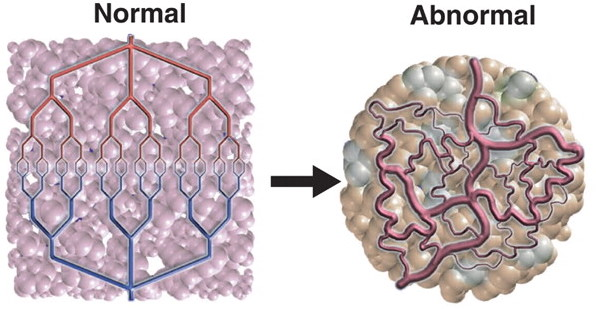
\includegraphics[width=0.65\textwidth]{images/BloodVessels.jpg}
\caption{\textit{Left, healthy vasculature. Right, tumour abnormal vasculature\cite{Jain58}} \label{BloodVessels}}
\end{figure}


\noindent To achieve this ambitious goal, a comprehensive understanding of the haemodynamics in micro- circulation is required for both the beginning and progression of the disease. However, it is very difficult to attain such knowledge solely through experiments due to the immense complexity of micro-circulatory blood flow in the human body. Furthermore, it still remains unclear how the different structural features of the micro-vessels and the components of blood (E.g. white blood cells, platelets etc; see Figure \ref{BloodComponents}) affect blood flow, tissue dysfunction and tumour growth. This also applies to finding out how these contributing factors can be exploited in disease therapy and other bio-engineering applications. Such complexity gives rise to major obstacles and challenges despite the recent technical advances in experimental techniques along with the breakthroughs made in developing animal models.\cite{PriesAR1994RtBF, Pries2000TheLayer, PRIES198981, Pries1992BloodHematocrit} \\

\noindent Recent computational techniques\cite{Noguchi14159, DoddiSaiK2009Tcmo, Freund2014, Balogh2018, 2020Charles} for blood flow modelling have developed rapidly and act as a powerful tool to analyse the micro-circulatory haemodynamics within complex geometries (E.g. flow distribution, RBC partitioning, haematocrit heterogeneity, wall shear stress difference). Such techniques have also become more reliable to validate some of the well-known blood flow phenomena (e.g. Zweifach-Fung effect, F{\aa}hr{\ae}us-Lindqvist effect and plasma skimming) observed in previous experimental studies. Furthermore, the recent technical advances in intravital microscopy and measurement techniques have accelerated the progress in characterising the blood flow behaviours in micro-circulations. However, it is still beyond our reach to attain a fully established model of the micro-circulatory blood flow including all biophysical or biochemical elements due to the constraints of computational power. \\

\noindent For this reason, several reduced-order models (ROM) were introduced to simplify the mathematical calculations and provide reliable predictions of haemodynamic quantities with satisfactory accuracy and lower computational expense. Various simplifications have also been made to existing models and some of the most common simplifications implemented were either dimensionality reduction or rheology homogenisation.\cite{CharlesPhDThesis2020} Dimensionality reduction relates to applying two-dimensional (2D) models to describe three-dimensional (3D) effects observed in \textit{in vivo} and \textit{in vitro}. Rheology homogenisation approximates blood flow as a homogeneous non-Newtonian fluid to simplify the intrinsic heterogeneity of blood arising from the non-continuum effects.\cite{CharlesPhDThesis2020} Another common simplification made is assuming negligible inertial effects due to low Reynolds number under Stokes flow regime in micro-circulations. 


\begin{figure}[H]
\centering
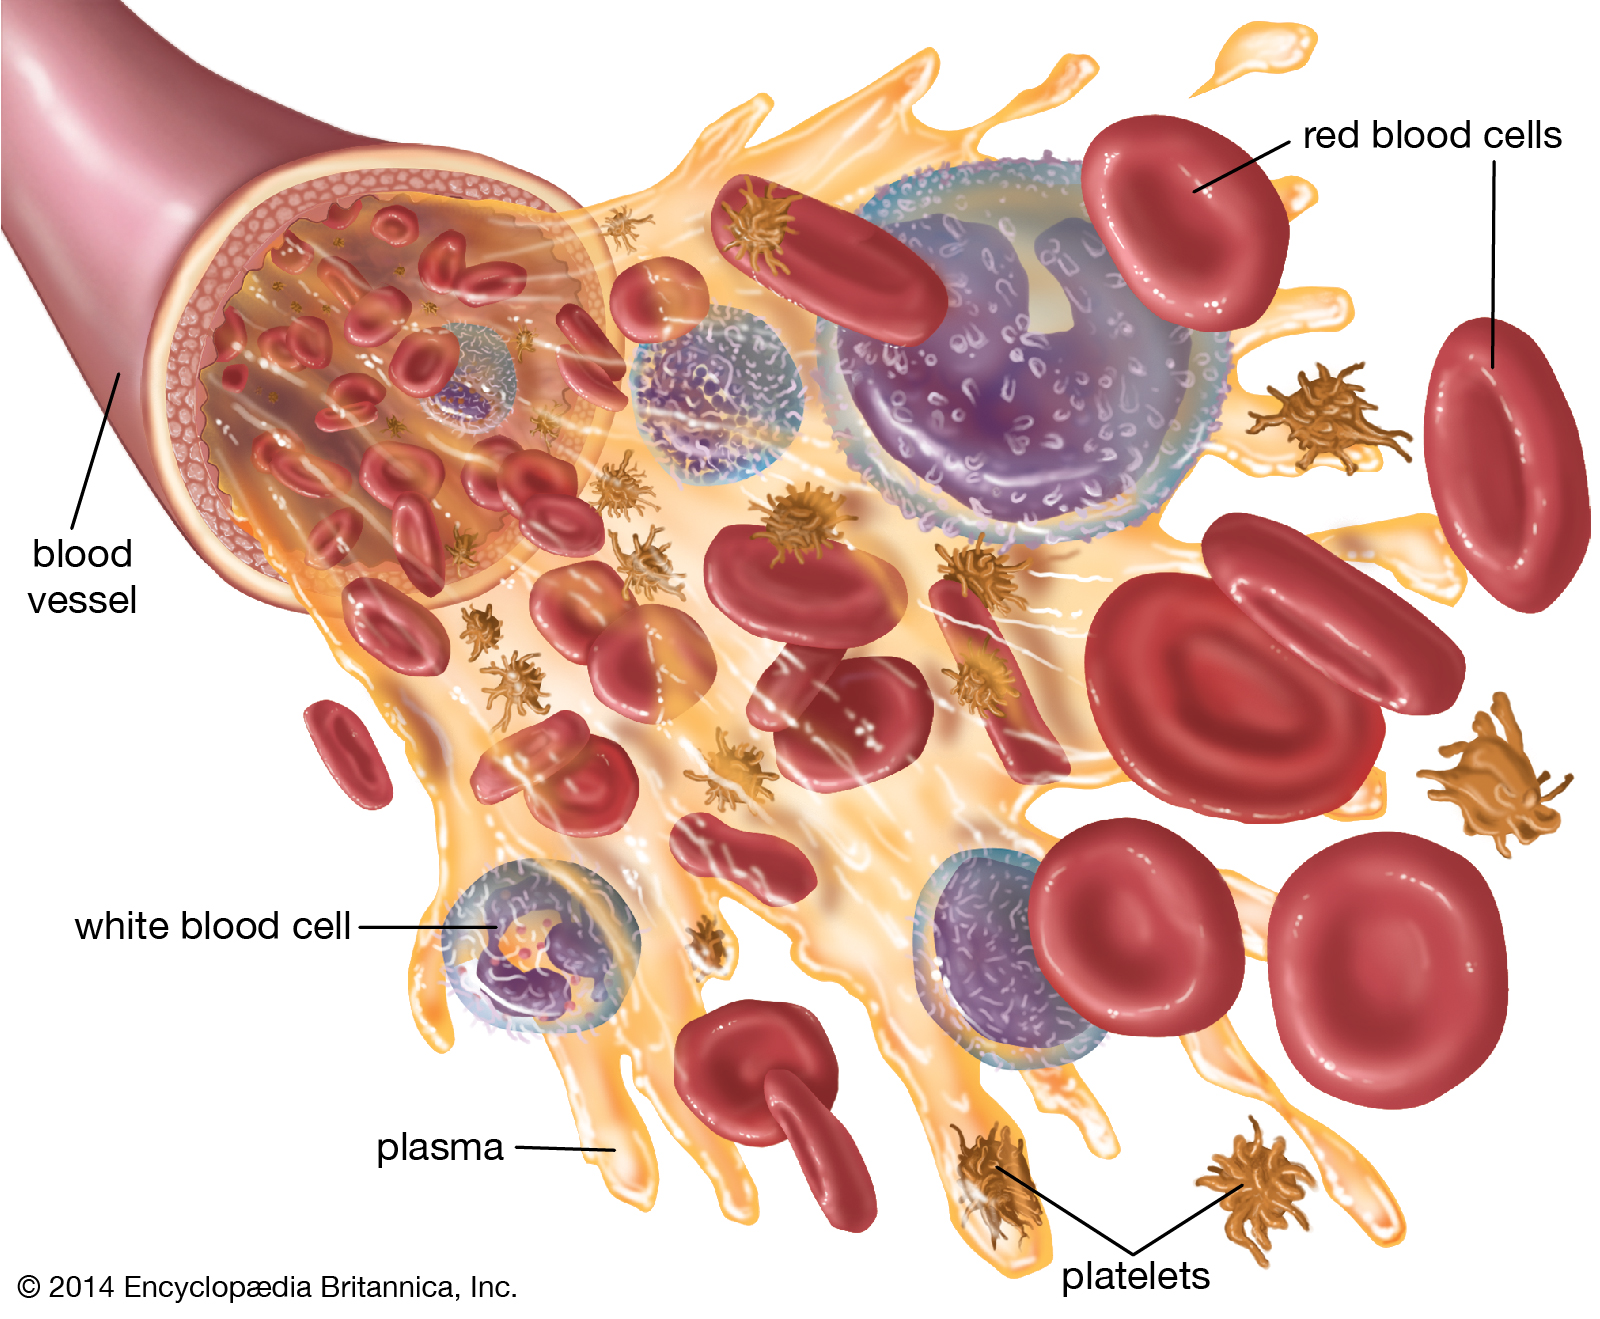
\includegraphics[width=0.65\textwidth]{images/BloodComponents.jpeg}
\caption{\textit{Blood is made up of multiple components, including red blood cells, white blood cells, platelets, and plasma. \cite{whitebloodcells}} \label{BloodComponents}}
\end{figure}


\noindent Despite decades of extensive research and theoretical studies in this field, multiple effects still remained unexplained from the predictions obtained in these simplified models (E.g. 2D models or continuum flow models). The conventional assumptions (E.g Poiseuille law, symmetrical haematocrit profile or time-average accuracy) also do not take into account certain key cellular characteristics of blood at micro-scale which affects the quantification of certain measuring flow variables like apparent viscosity and wall shear stress. Therefore, there are still significant challenges in quantitatively describing the micro-circulatory blood flow and pinpointing the potential haemodynamic mechanisms in micro-scale systems. \\


\noindent This brings us to the purpose of the current research project which is to analyse and identify the correlations from existing particle-based simulation data of blood flow in 3D complex microvascular networks.\cite{2020Charles} It was also investigated how well the predictions from some of the established ROMs developed by Pries et al.\cite{A.R.Pries2005Mbvi, PriesAR1994RtBF} are matched against simulation data in order to identify the existence of certain haemodynamic effects in the studied networks. Furthermore, distinct correlations were identified to take note of the contributing factors for the observed effects found from simulation data. This results to suggesting what are the next steps required to develop a reduced-order model that captures the observed effects on a network level in micro-circulations. Therefore, the overall work in this research project helps to provide a better understanding of the blood flow behaviours in micro-vessels based on fluid mechanical perspectives. 







